% !TEX root = ../main.tex

\section{Additional background}
\label{app:back}

\subsection{Ethereum and Blockchain Technology}
\label{app:ethback}

A public blockchain is an open peer-to-peer network that maintains a set of transactions without a single entity in charge. In Ethereum, \emph{transactions} encode the bytecode of user-written \emph{decentralized applications (DApps)} to be stored on the blockchain; and the function calls made to the DApp. Every execution of every function call is validated by all honest, participating nodes to correct; a property that is robust against a fraction of faulty and malicious network nodes (or more precisely, their accumulated computational power). Once transactions are agreed upon, all honest participants will have identical sets of transactions in the same order. For Ethereum, this is conceptualized as the current state of a large \emph{virtual machine (EVM)} that is running many DApps.

Transactions are broadcast by users to the blockchain network where they are propagated to all nodes. Nodes that choose to \emph{mine} will collect transactions (in the order of their choosing) into a block, and will attempt to have the network reach a consensus that their block should be added to the set (or chain) of previous blocks. A transaction is considered finalized once consensus on its inclusion has held for several additional blocks.

% JC: Should explain what "calldata" is as it is important for gas costs on Arbitrum

\subsubsection{Ethereum's Gas Model.} 

Every transaction results in the participating nodes having to execute bytecode. This is not free. When a transaction is executed, each opcode in the execution path accrues a fixed, pre-specified amount of \emph{gas}. The function caller will pledge to pay a certain amount of Ethereum's internal currency \emph{ETH} (typically quoted in units of Gwei which is one billionth of an ETH) per unit of gas, and miners are free to choose to execute that transaction or ignore it. The function caller is charged for exactly what the transaction costs to execute, and they cap the maximum they are willing to be charged (\textit{gas limit}). If the cap is too low to complete the execution, the miner keeps the Gwei and \emph{reverts} the state of the EVM (as if the function never ran).

A miner can include as many transactions (typically preferring transactions that bid the highest for gas) that can fit under a pre-specified \textit{block gas limit}, which is algorithmically adjusted for every block. As of the time of writing, the limit is approximately 11M gas. Essentially, our main research question is how many on-chain trades can be executed without exceeding that limit. Later, we also discuss several bytecode operations (\emph{opcodes}) that refund gas (\ie cost negative gas), which we heavily utilize in our optimizations.

\subsubsection{Gas Refunds.} 

In order to reconstruct the current state of Ethereum's EVM, a node must obtain a copy of every variable change since the genesis block (or a more recent `checkpoint' that is universally agreed to). For this reason, stored variables persist for a long time and, at first glance, it seems pointless to free up variable storage (and unclear what `free up' even means). Once the current state of the EVM is established by a node, it can forget about every historical variable changes and only concern itself with the variables that have non-zero value (as a byte string for non-integers) in the current state (uninitialized variables in Ethereum have the value 0 by default). Therefore, freeing up variables will reduce the amount of state Ethereum nodes need to maintain going forward.

For this reason, some EVM operations cost a negative amount of gas. That is, the gas is \textit{refunded} to the sender at the end of the transaction, however (1) the refund is capped at 50\% of the total gas cost of the transaction, and (2) the block gas limit applies to the pre-refunded amount (\ie a transaction receiving a full refund can cost up to 5.5M gas with an 11M limit). Negative gas operations include:

\begin{itemize}

\item \texttt{SELFDESTRUCT}. This operation destroys the contract that calls it and refunds its balance (if any) to a designated receiver address. The  \texttt{SELFDESTRUCT} operation does not remove the initial byte code of the contract from the chain. It always refunds 24,000 gas. For example, if contract A stores a single non-zero integer and contract B stores 100 non-zero integers, the \texttt{SELFDESTRUCT} refund for both is the same (24,000 gas).


\item \texttt{SSTORE}. This operation loads a storage slot with a value. Using \texttt{SSTORE} to load a zero into a storage slot with a non-zero value means the nodes can start ignoring it (recall that all variables, even if uninitialized, have zero by default). Doing this refunds 15,000 gas per slot.

\end{itemize}

At the time of this writing, Ethereum transaction receipts only account for the \texttt{gasUsed}, which is the total amount of gas units spent during a transaction, and users are not able to obtain the value of the EVM's refund counter from inside the EVM~\cite{signer2018gas}. So in order to account for refunds in  Tables~\ref{tab:PQUnitTests}, we calculate them manually. First, we determine exactly how many storage slots are being cleared or how many smart contracts are being destroyed, then we multiply these numbers by 24,000 or 15,000 respectively.

\subsubsection{Optimistic Roll-Ups.}
\label{app:rollup}


\begin{figure}[t]
\centering
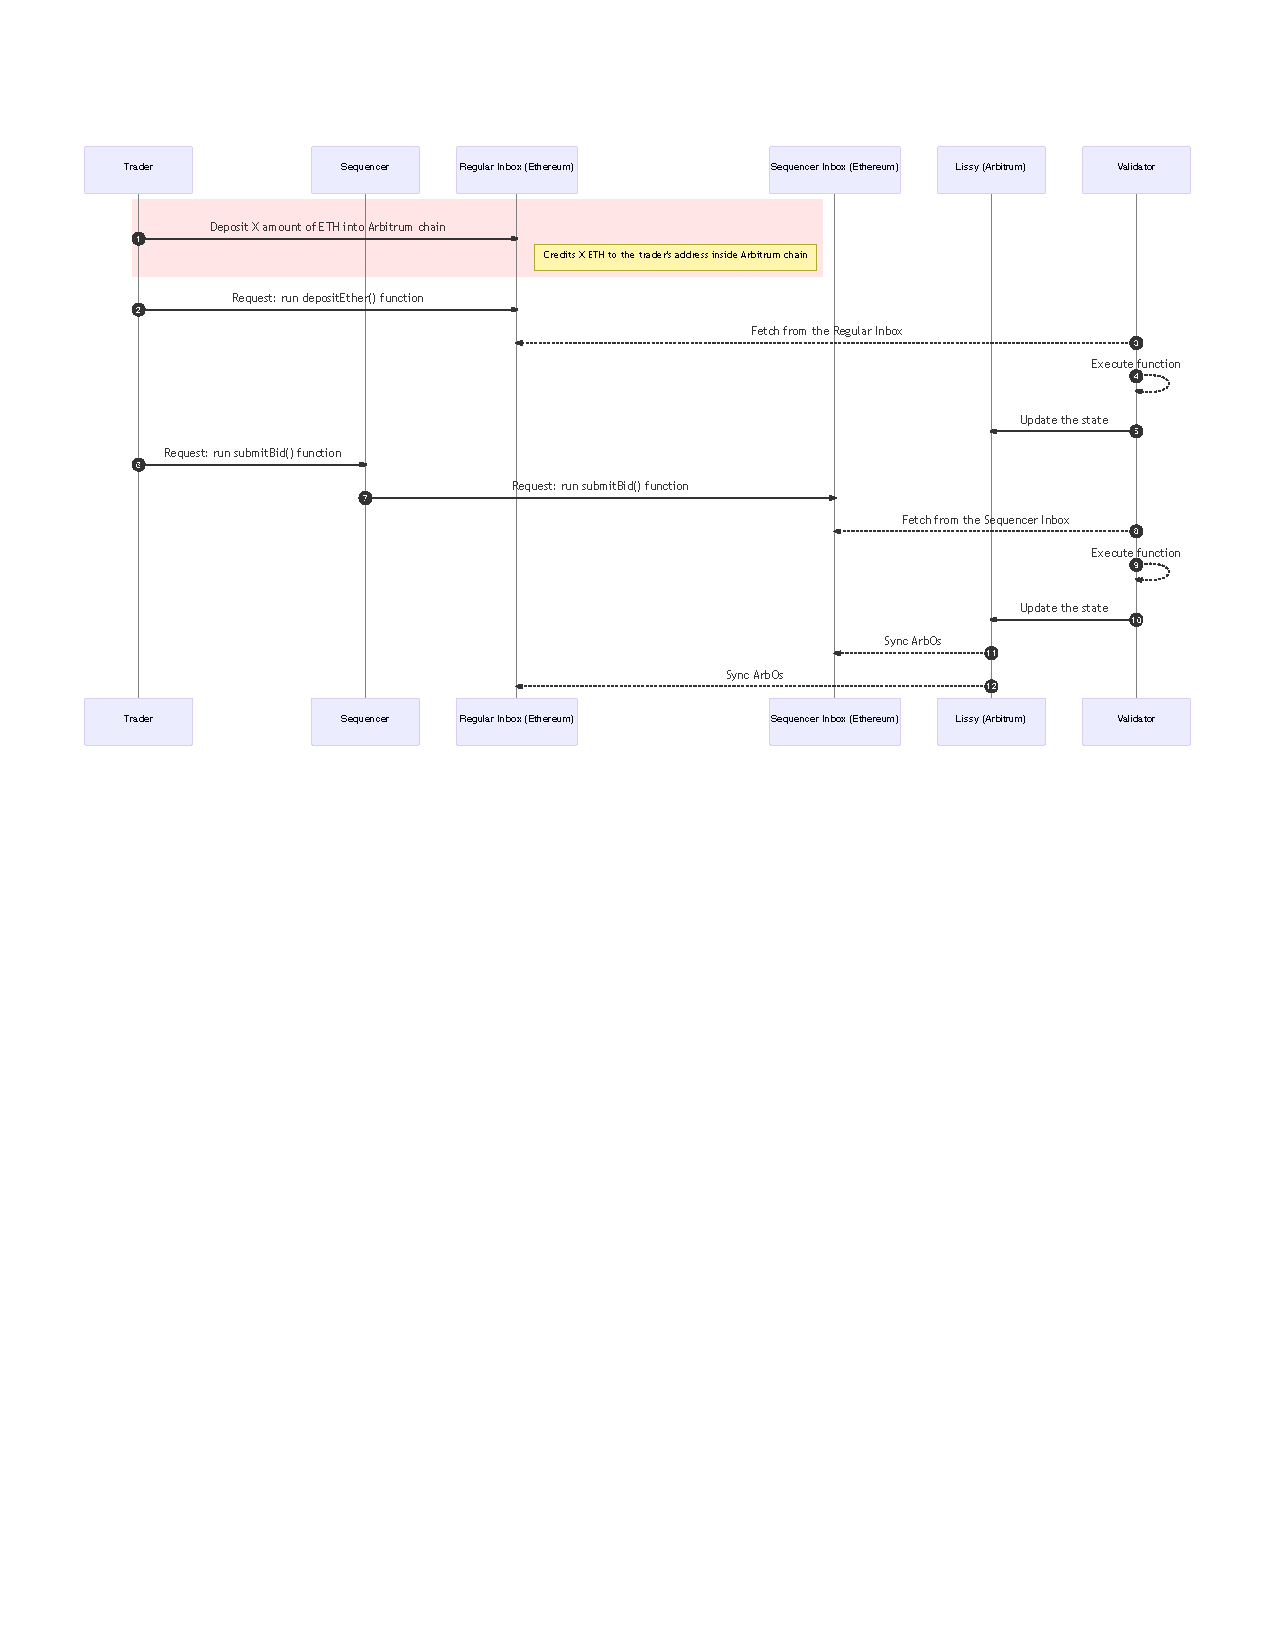
\includegraphics[width=1\textwidth]{fig/lissyL2.pdf}
\caption{\footnotesize{Overview of \cm on Arbitrum.}  \label{fig:lissyl2}}
\end{figure}


%We have avoided augmenting \cm with centralized components and third party services as our research question concerns the feasibility of a system with a minimum of regulatory hooks. However from a regulatory stance, there is a big difference between an architecture where the centralized component is publicly visible and interacted with by users (\eg most DEXes, roll-up architectures like Loopring, and commit-chain solutions like TEX). We consider an alternative design that is almost as difficult to regulate as a fully on-chain solution. In this design, an off-chain component is introduced to boost performance but it only interacts with the Ethereum network and never directly with traders. Traders still only interact with Ethereum.


\textit{Layer 2} solutions are a group of technologies that are designed and proposed to address specific drawbacks of executing transactions on \textit{Layer 1} (\ie Ethereum and other blockchains)~\cite{gudgeon2020sok}. These technologies focus on fast transaction throughput, reducing gas costs, or educing transaction latency. When using \cm, we strive to reduce the gas cost as performance is the main bottleneck. Thus, we choose a Layer 2 technology called \textit{roll-up} which aims at reducing the gas cost for operating on Layer 1 by taking the transaction executions off-chain and only using the Ethereum blockchain for storing data. In a roll-up, every transaction is executed by a server or cluster of servers known as \textit{validators} that can be run by a collection of users or third party operators (here they can be run by the token issuer). These validators then push the result of the executions (\ie updates in the EVM state) back to the Ethereum and assure the Ethereum network that the transactions have been executed correctly.

A function can be computed off-chain and the new state of the DApp, called a \textit{rollup}, is written back to the blockchain, accompanied by either (1) a proof that the function was executed correctly, or (2) a dispute resolution process that can resolve, on-chain, functions that are not executed correctly (\eg Arbitrum~\cite{kalodner2018arbitrum}). In the case of (1), validating the proof must be cheaper than running the function itself. There are two main approaches: (1a) the first is to use cryptographic proof techniques (\eg SNARKS~\cite{BCGTV13,GGPR13} and variants~\cite{BBHR19}). This is called a \textit{zk-rollup}. Note that the proofs are heavy to compute (introducing a burden to the validators who generate them) but considered valid once posted to the Ethereum. The second approach (1b) is to execute the function in a trusted execution environment (TEE; \eg Intel SGX) and validate the TEE's quote on-chain (\eg Ekiden~\cite{cheng2019ekiden}).\footnote{The TEE-based approach is mired by recent attacks on SGX~\cite{SGX1,SGX2,SGX3,SGX4}, however these attacks do not necessarily apply to the specifics of how SGX is used here, and safer TEE technologies like Intel TXT (\cf~\cite{ZBC+19}) can be substituted.} Approach (2) is called an \textit{optimistic roll-up}. Although the dispute time delays result in a slower transaction finality, optimistic roll-ups substantially increase the performance by decreasing the gas cost. 

Arbitrum and Ethereum Optimism are the two prominent deployments of an optimistic roll-up. Arbitrum  uses a multi-round dispute process that results in very minimal L1 gas costs to resolve a dispute. Specifically, if a dispute over a transaction arrises, the L1 cost of resolving the dispute is a small fraction of the cost of executing the transaction itself (whereas in Optimism, the dispute resolution cost is essentially the same as executing the transaction). 

Our \cm variant is not the first roll-up-based order book. Loopring 3.0\footnote{\url{https://loopring.org}} offers a continuous-time order book. The primary difference is that orders in Loopring 3.0 are submitted off-chain to the operator directly, whereas our variant uses on-chain submission so that the roll-up server does not need to be publicly reachable. Loopring 3.0 can operate near high-frequency trading as order submission is unhampered by Ethereum. However, its  roll-up proof does not ensure that the exchange did not reorder transactions, which is particularly problematic in a continuous-time order book. Traders who prioritize trade fairness might opt for a solution like our variant, while traders who want speed would vastly prefer the Loopring architecture which offers near-CEX speed while being non-custodial. Loopring leaves a regulatory hook whereas our variant could be nearly as difficult to regulate as a fully on-chain solution if the roll-up server was kept anonymous: Ethereum and Arbitrum themselves would be the only regulatory hooks.


\subsection{Trade Execution Systems}
\label{app:markets}

\paragraph{Centralized Exchanges (CEX).} Traditional financial markets (\eg NYSE and NASDAQ) use order-matching systems to arrange trades. An exchange will list one or more assets (stocks, bonds, derivatives, or more exotic securities) to be traded with each other, given its own order book priced in a currency (\eg USD). Exchanges for blockchain-based assets (also called crypto assets by enthusiasts) can operate the same way, using a centralized exchange (CEX) design where a firm (\eg Binance, Bitfinex, \etc) operates the platform as a trusted third party in every aspect: custodianship over assets/currency being traded, exchanging assets fairly, offering the best possible price execution. Security breaches and fraud in centralized exchanges  (\eg MtGox~\cite{TheHisto45:online}, QuadrigaCX~\cite{SEBIOrde83:online}, and many others) have become a common source of lost funds for users, while accusations of unfair trade execution have been levelled but are difficult to prove. Today, CEXes are often regulated as other money service businesses---this provides some ability for the government to conduct financial tracking but does little to provide consumer protection against fraud.

\paragraph{On-chain Order Books.} For trades between two blockchain-based assets (\eg a digital asset priced in a cryptocurrency, stablecoin, or second digital asset), order matching can be performed `on-chain' by deploying the order-matching system either on a dedicated blockchain or inside a decentralized application (DApp). In this model, traders entrust their assets to an autonomously operating DApp with known source code instead of a third party custodian that can abscond with or lose the funds. The trading rules will operate as coded, clearing and settling can be guaranteed, and order submission is handled by the blockchain---a reasonably fair and transparent system (but see front-running below). Finally, anyone can create an on-chain order book for any asset (on the same chain) at any time. While these sound ideal, performance is a substantial issue and the main subject of this paper. Since it is an open system, there is no obvious regulatory hook (beyond the blockchain itself).

In this paper, we focus on benchmarking an order book for the public blockchain Ethereum. Ethereum is widely used and we stand to learn the most from working in a performance-hostile environment. Exchanges could be given their own dedicated blockchain, where trade execution logic can be coded into the network protocol. Trading systems on permissioned blockchains (\eg NASDAQ Linq, tZero) can also improve execution time and throughput, but they reduce user transparency and trust if unregulated.

\paragraph{On-chain Dealers.} An advantage of on-chain trading is that other smart contracts, not just human users, can initiate trades, enabling broader decentralized finance (DeFi) applications. This has fuelled a resurgence in on-chain exchange but through a quote-driven design rather than an order-driven one. Automated market makers  (\eg Uniswap v3) have all the trust advantages of an on-chain order book, plus they are relatively more efficient. The trade-off is that they operate as a dealer---the DApp exchanges assets from its own inventory. This inventory is loaded into the DApp by an investor who will not profit from the trades themselves but hopes their losses (termed `impermanent losses') are offset over the long-term by trading fees. By contrast, an order book requires no upfront inventory and trading fees are optional. Finally, there is a complicated difference in their price dynamics (\eg market impact of a trade, slippage between the best bid/ask and actual average execution price, \etc)---deserving of an entire research paper to precisely define. We leave it as an assertion that with equal liquidity, order books have more favorable price dynamics for traders.

\paragraph{Hybrid Designs.} Before on-chain dealers became prominent in the late 2010s, the most popular design was hybrid order-driven exchanges with some trusted off-chain components and some on-chain functionalities. Such decentralized exchanges (DEXes) were envisioned as operating fully on-chain, but performance limitations drove developers to move key components, such as the order matching system, off-chain to a centralized database. A landscape of DEX designs exist (\eg EtherDelta, 0x, IDEX, \etc): many avoid taking custodianship of assets off-chain, and virtually all (for order-driven markets) operate the order book itself off-chain (a regulatory hook). A non-custodial DEX solves the big issue of a CEX---the operator stealing the funds---however trade execution is still not provably fair, funds can still be indirectly stolen by a malicious exchange executing unauthorized trades, and server downtime is a common frustration for traders. An enhancement is to prove that trade execution is correct (\eg Loopring) but these proofs have blind spots (discussed above in Appendix~\ref{app:rollup}).

\subsection{Call Markets}
\label{app:cm}
\begin{itemize}
\item The call market first Matches Alice ask order to sell 1 at 10 with Eric's bid order to Buy 3 at 12. The trader happens at the price Alice asks for; 10, and 2 will be given to the miner as a price improvement. This trade fills Alice's order and leaves Eric with a remainder of 2 to buy at 12. 
\item Next, the call market matches Eric's remainder of 2 with the next highest priority ask order in the list which is Bob's order to sell 4 at 10.15. Trade occurs at 10.15 and 1.85 will be given to the miner as a price improvement. This trade fills the remainder of Eric's bid order and leaves Bob with a remainder of 2 to sell at 10.15.
\item The market now matches the next highest bid order in the list, Alex's bid order to buy 1 at 12.15, with the remainder of Bob's ask order to sell 2 at 10.15. Trader occurs at 10.15 and 2 will be given to minder as a price improvement. This trader fills Alex bis order and leaves Bob with a remainder of 1 to sell at 10.15.
\item Next, the market matches Adam's bid order to buy 3 at 13 with the remainder of Bob's ask order to sell 1 at 10.15. Trade occurs at 10.15 and 2.85 will be given to miner as a price improvement. This match fills the Bob order and leaves Adam with a remainder of 2 to buy at 13.
\item The market then matches Sam's ask order to sell 4 at 10.18 with the remainder of Adam's bid order to buy 2 at 13. Trade occurs at 10.18 and 2.82 is given to miner as a price improvement. This trade fills Adam's order and leaves Sam with a remainder of 2 to sell at 10.18 unfilled. 
\end{itemize}

\section{Cleaning-Up Revisited: Clearing Mappings}
\label{app:clean}

Beyond the cleaning up issues with priority queues in Section~\ref{sec:gasrefund}, \cm also uses mappings with each market. Traders preload their account with tokens to be traded (which comply with a common token standard called ERC20) and/or ETH. \cm tracks what they are owed using a mapping called \texttt{totalBalance} and allows traders to withdraw their tokens at any time. However if a trader submits an order (\ie ask for their tokens), the tokens are committed and not available for withdrawal until the market closes (after which, the balances are updated for each trade that is executed). Committed tokens are also tracked in a mapping called \texttt{unavailableBalance}. Sellers can request a token withdrawal up to their total balance subtracted by their unavailable balance.

As the DApp runs \texttt{closeMarket()}, it starts matching the best bids to the best asks. As orders execute, \texttt{totalBalance} and \texttt{unavailableBalance} are updated. At a certain point, the bids and asks will stop matching in price. At this point, every order left in the order book cannot execute (because the priority queue sorts orders by price, and so orders deeper in the queue have worst prices than the order at the head of the queue). Therefore all remaining entries in \texttt{unavailableBalance} can be cleared.

In Solidity, it is not possible to delete an entire mapping without individually zeroing out each entry key-by-key. At the same time, it is wasteful to let an entire mapping sit in the EVM when it will never be referenced again. The following are some options for addressing this conflict.

\begin{enumerate}

\item \textbf{Manually Clearing the Mapping.} Since mappings cannot be iterated, a common design pattern used by DApp developers is to store keys in an array and iterate over the array to zero out each mapping and array entry. Clearing a mapping this way costs substantially more to clear than what is refunded.

\item \textbf{Store the Mapping in a Separate DApp.} We could wrap the mapping inside its own DApp and when we are done with the mapping, we can run \texttt{SELFDESTRUCT} on the contract. This refunds us 24,000 gas which is less than the cost of deploying the extra contract. Additionally, every call to the mapping is more expensive because (1) it is an external function call, and (2) the calls need access control to ensure only the market contract can write to it (if a mapping is a local variable, you get private access for free). 

\item \textbf{Leave and Ignore the Mapping.} The final option is to not clear the mapping and just create a new one (or create a new prefix for all mapping keys to reflect the new version of the mapping). Unfortunately, this is the most economical option for DApp developers even if it is the worst option for Ethereum nodes. 

\end{enumerate}

Clearing storage is important for reducing EVM bloat. The Ethereum refund model should be considered further by Ethereum developers to better incentivize developers to be less wasteful in using storage. 

% = = = = = = = 
% = = = = = = = 
% = = = = = = = 

\section{Collateralization Options in Call Markets}
\label{app:collateral}

in \cm, both the tokens and ETH that a trader wants to potentially use in the order book are pre-loaded into the contract. Consider Alice, who holds a token and decides she wants to trade it for ETH. In this model, she must first transfer the tokens to the contract and then submit an ask order. If she does this within the same block, there is a chance that a miner will execute the ask before the transfer and the ask will revert. If she waits for confirmation, this introduces a delay. This delay seems reasonable but we point out a few options it could be addressed:

\begin{enumerate}

\item \textbf{Use \texttt{msg.value}.} For the ETH side of a trade (\ie for bids), ETH could be sent with the function call to \texttt{submitBid()} to remove the need for    \texttt{depositEther()}. This works for markets that trade ERC20 tokens for ETH, but would not work for ERC20 to ERC20 exchanges.

\item \textbf{Merge Deposits with Bids/Asks.} \cm could have an additional function that atomically runs the functionality of \texttt{depositToken()} followed by the functionality of \texttt{submitAsk()}. This removes the chance that the deposit and order submission are ordered incorrectly.

\item \textbf{Use ERC20 Approval.} Instead of \cm taking custody of the tokens, the token holder could simply approve \cm to transfer tokens on her behalf. If \cm is coded securely, it is unconcerning to allow the approval to stand long-term and the trader never has to lock up their tokens in the DApp. The issue is that there is no guarantee that the tokens are actually available when the market closes (\ie Alice can approve a DApp to spend 100 tokens even if she only has 5 tokens or no tokens). In this case, \cm would optimistically try to transfer the tokens and if it fails, move onto the next order. This also gives Alice an indirect way to cancel an order, by removing the tokens backing the order---this could be a feature or it could be considered an abuse.

\item \textbf{Use a Fidelity Bond.} Traders could post some number of tokens as a fidelity bond, and be allowed to submit orders up to 100x this value using approve. If a trade fails because the pledged tokens are not available, the fidelity bond is slashed as punishment. This allows traders to side-step time-consuming transfers to and from \cm while still incentivizing them to ensure that submitted orders can actually be executed. The trade-off  is that \cm needs to update balances with external calls to the ERC20 contract instead of simply updating its internal ledger.

\end{enumerate}

\section{Market Clearing Prices}

% JC: Not part of design landscape, find a new home for it

Call markets are heralded for fair price discovery. This is why many exchanges use a call market at the end of the day to determine the closing price of an asset, which is an important price both optically (it is well-published) and operationally (many derivatives settle based on the closing price). We purposely do not compute a `market clearing price' with \cm because miners can easily manipulate the price (\ie include a single wash trade at the price they want fixed), although they forgo profit for doing so. This is not merely hypothetical---Uniswap (the prominent quote-drive, on-chain exchange) prices have been manipulated to exploit other DeFi applications relying on them. Countermeasures to protect Uniswap price integrity could also apply to \cm: (1) taking a rolling median of prices over time, and (2) using it alongside other sources for the same price and forming a consensus. While \cm does not emit a market clearing price, it can be computed by a web application examining the order book at market close.